\documentclass[11pt]{amsart}
%%% WARNING: Do NOT change the page size, fonts, or margins!  Penalties will apply.

\usepackage{graphicx, hyperref}
\usepackage{amssymb,amsmath,amsthm, mathtools}
\usepackage{placeins} %enables \FloatBarrier, that prevents floats from going below it.
\usepackage{caption}
\usepackage{subcaption}
\usepackage{algpseudocode, algorithm}
\usepackage{tikz}
\usepackage{physics}
\usepackage[T1]{fontenc}
\usepackage{DejaVuSansMono}
\usetikzlibrary{arrows}
\usetikzlibrary{tikzmark}
\usepackage{listings}

% Define style for Python code snippets
\lstset{
    language=Python,
    basicstyle=\small\ttfamily, % Set font size to small
    frame=single, % Add frame around code snippets
    showstringspaces=false % Don't show spaces in strings
}

%%% WARNING: Do NOT change the page size, fonts, or margins!  Penalties will apply.
%%% WARNING: Do NOT change the page size, fonts, or margins!  Penalties will apply.

% Some macros for ease of use
\newcommand{\R}{{\mathbb R}}
\newcommand{\A}{{\mathrm{A}}}


\begin{document}
\title{Helping the Spacing Guild Navigate to Arrakis}
\author{Spencer Ashton, Curtis Evans, Cannon Tuttle, Tyler Sanders}

%% comment out next command to put today's date after names of group members, or put a desired day in the parethesis
\date{\today}

\begin{abstract}
    We find the optimal path and control of navigating from one planet to another planet by using the laws of gravity to help with 
    the acceleration. This is done by using Pontryagin maximum principle, and we discovered sensitivity in our system when optimizing over $t_f$ and found a solution to numerical instabilty when 
    adding massive planets such as the sun. 
\end{abstract}

\maketitle

%% First Section
\section{Background}
The \textbf{Dune} Guild Naviators are tasked with delivering House Atreides from the planet Caladan to Arrakis. Usually they solve the optimal control in their mind while taking spice, but since spice production
has been disrupted they've instead decided to turn to ACME students on Earth to solve the optimal control for them. They have asked the ACME students to find the best path while minimizing fuel consumption. 


\section{Mathematical Representation}
We used Newton's second law of motion $F=ma$ to arrive at our state equations where $m_p$ is the mass of the planet, $\mathbf{x}_s$ is the $x$ and $y$ position of the space ship, and $\mathbf{x}_p$ is the $x$
and $y$ position of the planet, and $\mathbf{u}$ is the acceleration in the $x$ and $y$ direction for the spaceship. We will have a set of planets $P = \{p_1, p_2,\dots,p_n\}$. \textcolor{red}{TODO} talk about what $G$ is and how this equation makes sense.
\[\ddot{\mathbf{x}} = -G\sum_{p\in{P}}^{}\frac{m_p}{||\mathbf{x}_s-\mathbf{x}_p||_2^3}(\mathbf{x}_s-\mathbf{x}_p) + \mathbf{u}\]
Converting $\ddot{\mathbf{x}}$ into a first order differential equation we get the following state equation. 
\[\begin{pmatrix}
    \dot{x}_s \\
    \dot{y}_s \\
    \ddot{x}_s\\
    \ddot{y}_s 
\end{pmatrix} = \begin{pmatrix}
    \dot{x}_s \\
    \dot{y}_s \\
    -G\sum_{p\in{P}}^{}\frac{m_p(x_s - x_p)}{((x_s-x_p)^2+(y_s-y_p)^2)^{3/2}} + u_x \\
    -G\sum_{p\in{P}}^{}\frac{m_p(y_s - y_p)}{((x_s-x_p)^2+(y_s-y_p)^2)^{3/2}} + u_y
\end{pmatrix}\]

We decided to minimize the control used to get the optimal fuel usage. That gives us the following cost functional and boundary conditions. 
\[J[u] = \int_{0}^{t_f}||\mathbf{u}||_2^2dt\]
\[\mathbf{x}_s(0) = \text{Caladan's Position},\: \dot{\mathbf{x}}_s(0) = \text{Caladan's Velocity}\]
\[\mathbf{x}_s(t_f) = \text{Arrakis' Position},\: \dot{\mathbf{x}}_s(t_f) = \text{Arrakis' Velocity}\]

\section{Solution}
We are now ready to use Pontryagin's maximum principle with 
\[H = \mathbf{p}\cdot\mathbf{f(\mathbf{x})} - L\]
Applying this to our state equation and Lagrangian we get the following Hamiltonian.
\[H = p_1\dot{x}_s + p_2\dot{y}_s + p_3\left[-G\sum_{p\in{P}}^{}\frac{m_p(x_s - x_p)}{((x_s-x_p)^2+(y_s-y_p)^2)^{3/2}} + u_x\right]\]
\[+ p_4\left[-G\sum_{p\in{P}}^{}\frac{m_p(y_s - y_p)}{((x_s-x_p)^2+(y_s-y_p)^2)^{3/2}} + u_y\right] - u_x^2 - u_y^2\]

This give us the following co-state evolution equations by using $\mathbf{p}' = -\frac{DH}{D\mathbf{x}}$
\begin{align*}
    \dot{p}_1 &= p_3G\left(\sum_{p\in{P}}^{}\frac{m_p}{((x_s-x_p)^2+(y_s-y_p)^2)^{3/2}} - \frac{3m_p(x_s - x_p)^2}{((x_s-x_p)^2+(y_s-y_p)^2)^{5/2}}\right) \\
    \dot{p}_2 &= p_4G\left(\sum_{p\in{P}}^{}\frac{m_p}{((x_s-x_p)^2+(y_s-y_p)^2)^{3/2}} - \frac{3m_p(y_s - y_p)^2}{((x_s-x_p)^2+(y_s-y_p)^2)^{5/2}}\right) \\
    \dot{p}_3 &= -p_1 \\
    \dot{p}_4 &= -p_2. \\
    p_1&(t_f)= p_2(t_f) = 0 = p_3(t_f) = p_4(t_f)
\end{align*}
Now we need to find $\tilde{\mathbf{u}}$ by maximizing the Hamiltonian i.e. $\frac{DH}{D\mathbf{u}} = 0$.
\[\frac{\partial H}{\partial u_x} = p_3 - 2u_x \:\:\text{and}\:\: \frac{\partial H}{\partial u_y} = p_4 - 2u_y\]
now solving for $u_x$ and $u_y$ we get
\[\tilde{u}_x = \frac{p_3}{2} \:\:\text{and}\:\: \tilde{u}_y = \frac{p_4}{2}.\]
Plugging $\tilde{u}_x$ and $\tilde{u}_y$ back into the state and costate evolution equations we get the following boundary value problem.

\begin{align*}
    \dot{x}_s &= \dot{x}_s \\
    \dot{y}_s &= \dot{y}_s \\
    \ddot{x}_s &= -G\sum_{p\in{P}}^{}\frac{m_p(x_s - x_p)}{((x_s-x_p)^2+(y_s-y_p)^2)^{3/2}} + \frac{p_3}{2} \\
    \ddot{y}_s &= -G\sum_{p\in{P}}^{}\frac{m_p(y_s - y_p)}{((x_s-x_p)^2+(y_s-y_p)^2)^{3/2}} + \frac{p_4}{2} \\
    \dot{p}_1 &= p_3G\left(\sum_{p\in{P}}^{}\frac{m_p}{((x_s-x_p)^2+(y_s-y_p)^2)^{3/2}} - \frac{3m_p(x_s - x_p)^2}{((x_s-x_p)^2+(y_s-y_p)^2)^{5/2}}\right) \\
    \dot{p}_2 &= p_4G\left(\sum_{p\in{P}}^{}\frac{m_p}{((x_s-x_p)^2+(y_s-y_p)^2)^{3/2}} - \frac{3m_p(y_s - y_p)^2}{((x_s-x_p)^2+(y_s-y_p)^2)^{5/2}}\right) \\
    \dot{p}_3 &= -p_1 \\
    \dot{p}_4 &= -p_2. \\
\end{align*}
With boundary conditions
\[x_s(t_0) = x_{p_1}(t_0),\:y_s = y_{p_1}(t_0),\:\dot{x}_s(t_0) = \dot{x}_{p_1}(t_0),\:\dot{y}_s(t_0) = \dot{y}_{p_1}(t_0)\]
and 
\[x_s(t_f) = x_{p_2}(t_f),\:y_s = y_{p_2}(t_f),\:\dot{x}_s(t_f) = \dot{x}_{p_2}(t_f),\:\dot{y}_s(t_f) = \dot{y}_{p_2}(t_f)\]
if we are optimizing over $t_f$ we get the added boundary condition that $H(t_f) = 0$, and if we are optimizing over $t_0$ we get $H(t_0)=0$. This problem is now set up to use \lstinline{solve_bvp}.

\section{Solution}
We hope to acheive an optimal path from Caladan to Arrakis with a fixed final time, a free final time where we need $H(t_f) = 0$ as an added boundary condition, and an optimal control
with multiple solar systems and planets. We also want to figure out the best path with a given arbitrary layout for a given solar system. Essentially the Spacing Guild would like to use 
our algorithms to help navigate from any planet. \textcolor{red}{TODO} should we talk about optimizing over $t_0$ if so we should say. We realize that in planetary travel we would like to 
get to a given planet on a fixed day and then leave our leaving day free. That would mean we are optimixing over $t_0$ so we would have a free parameter with the added boundary condition that
$H(t_0) = 0$.

\subsection{Fixed End Position}

We simulated our model using the inner planets of our own solar system, but changed the names to be planets from the \textbf{Dune} universe so the Guild Naviators wouldn't be confused.
The first model we ran was without the sun and a fixed final time of $200$ Earth days (See Figure \ref{fig:fixed_time_no_sun}). 

\begin{figure}[htp]
    \centering
    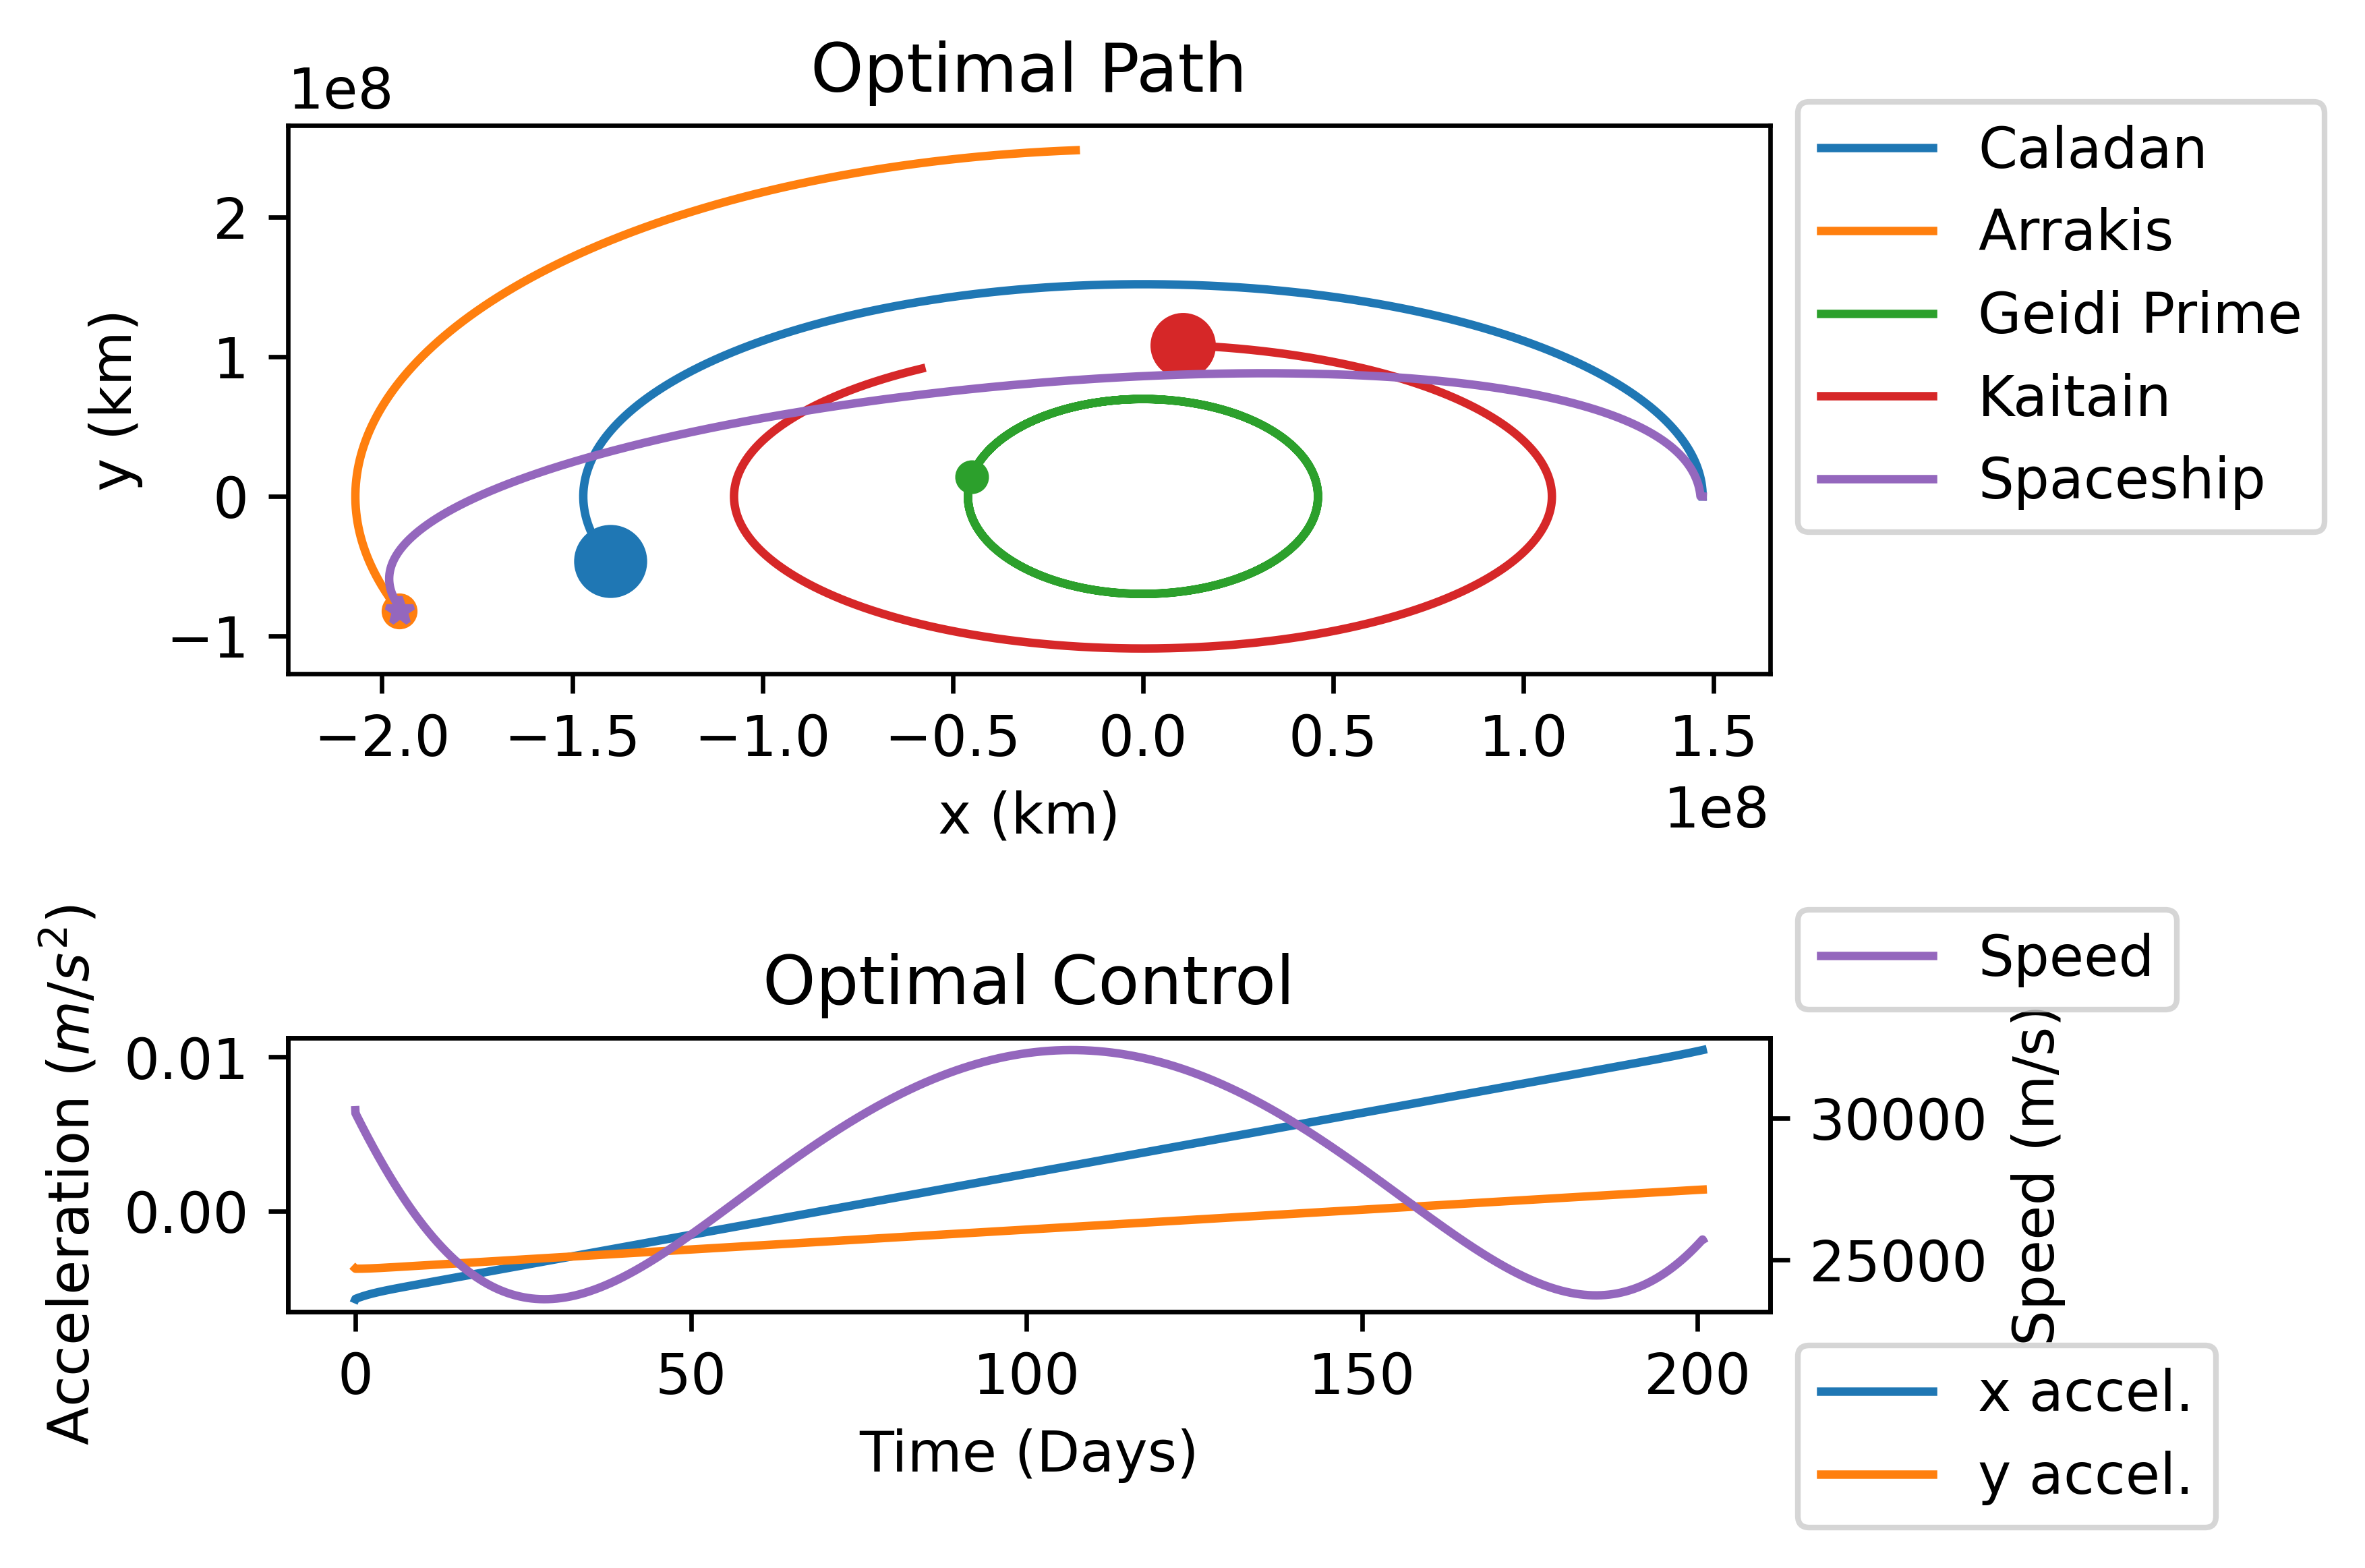
\includegraphics[width=0.8\textwidth]{f2.png}\hfill
    \caption{Going from Caladan to Arrakis in 200 Earth Days with a fixed final time}
    \label{fig:fixed_time_no_sun}
\end{figure}

\subsection{Free Final Time}

Our bare bones model got us from Caladan to Arrakis successfully, but we would like to save as much fuel as possible so our main goal is to minimize over $t_f$ as well. This was done by 
adding a free parameter in \lstinline{solve_bvp} and adding the boundary condition of $H(t_f) = 0$. We discovered that this model was sensitive to initial guess of $t_f$ and also the initial
state space guess. We ran model with varying $t_f$ guesses and got varying results with no convergence on an optimal $t_f$ for all the different guesses (See Figure \ref{fig:free_time_no_sun}). 

\begin{figure}[htp]
    \centering
    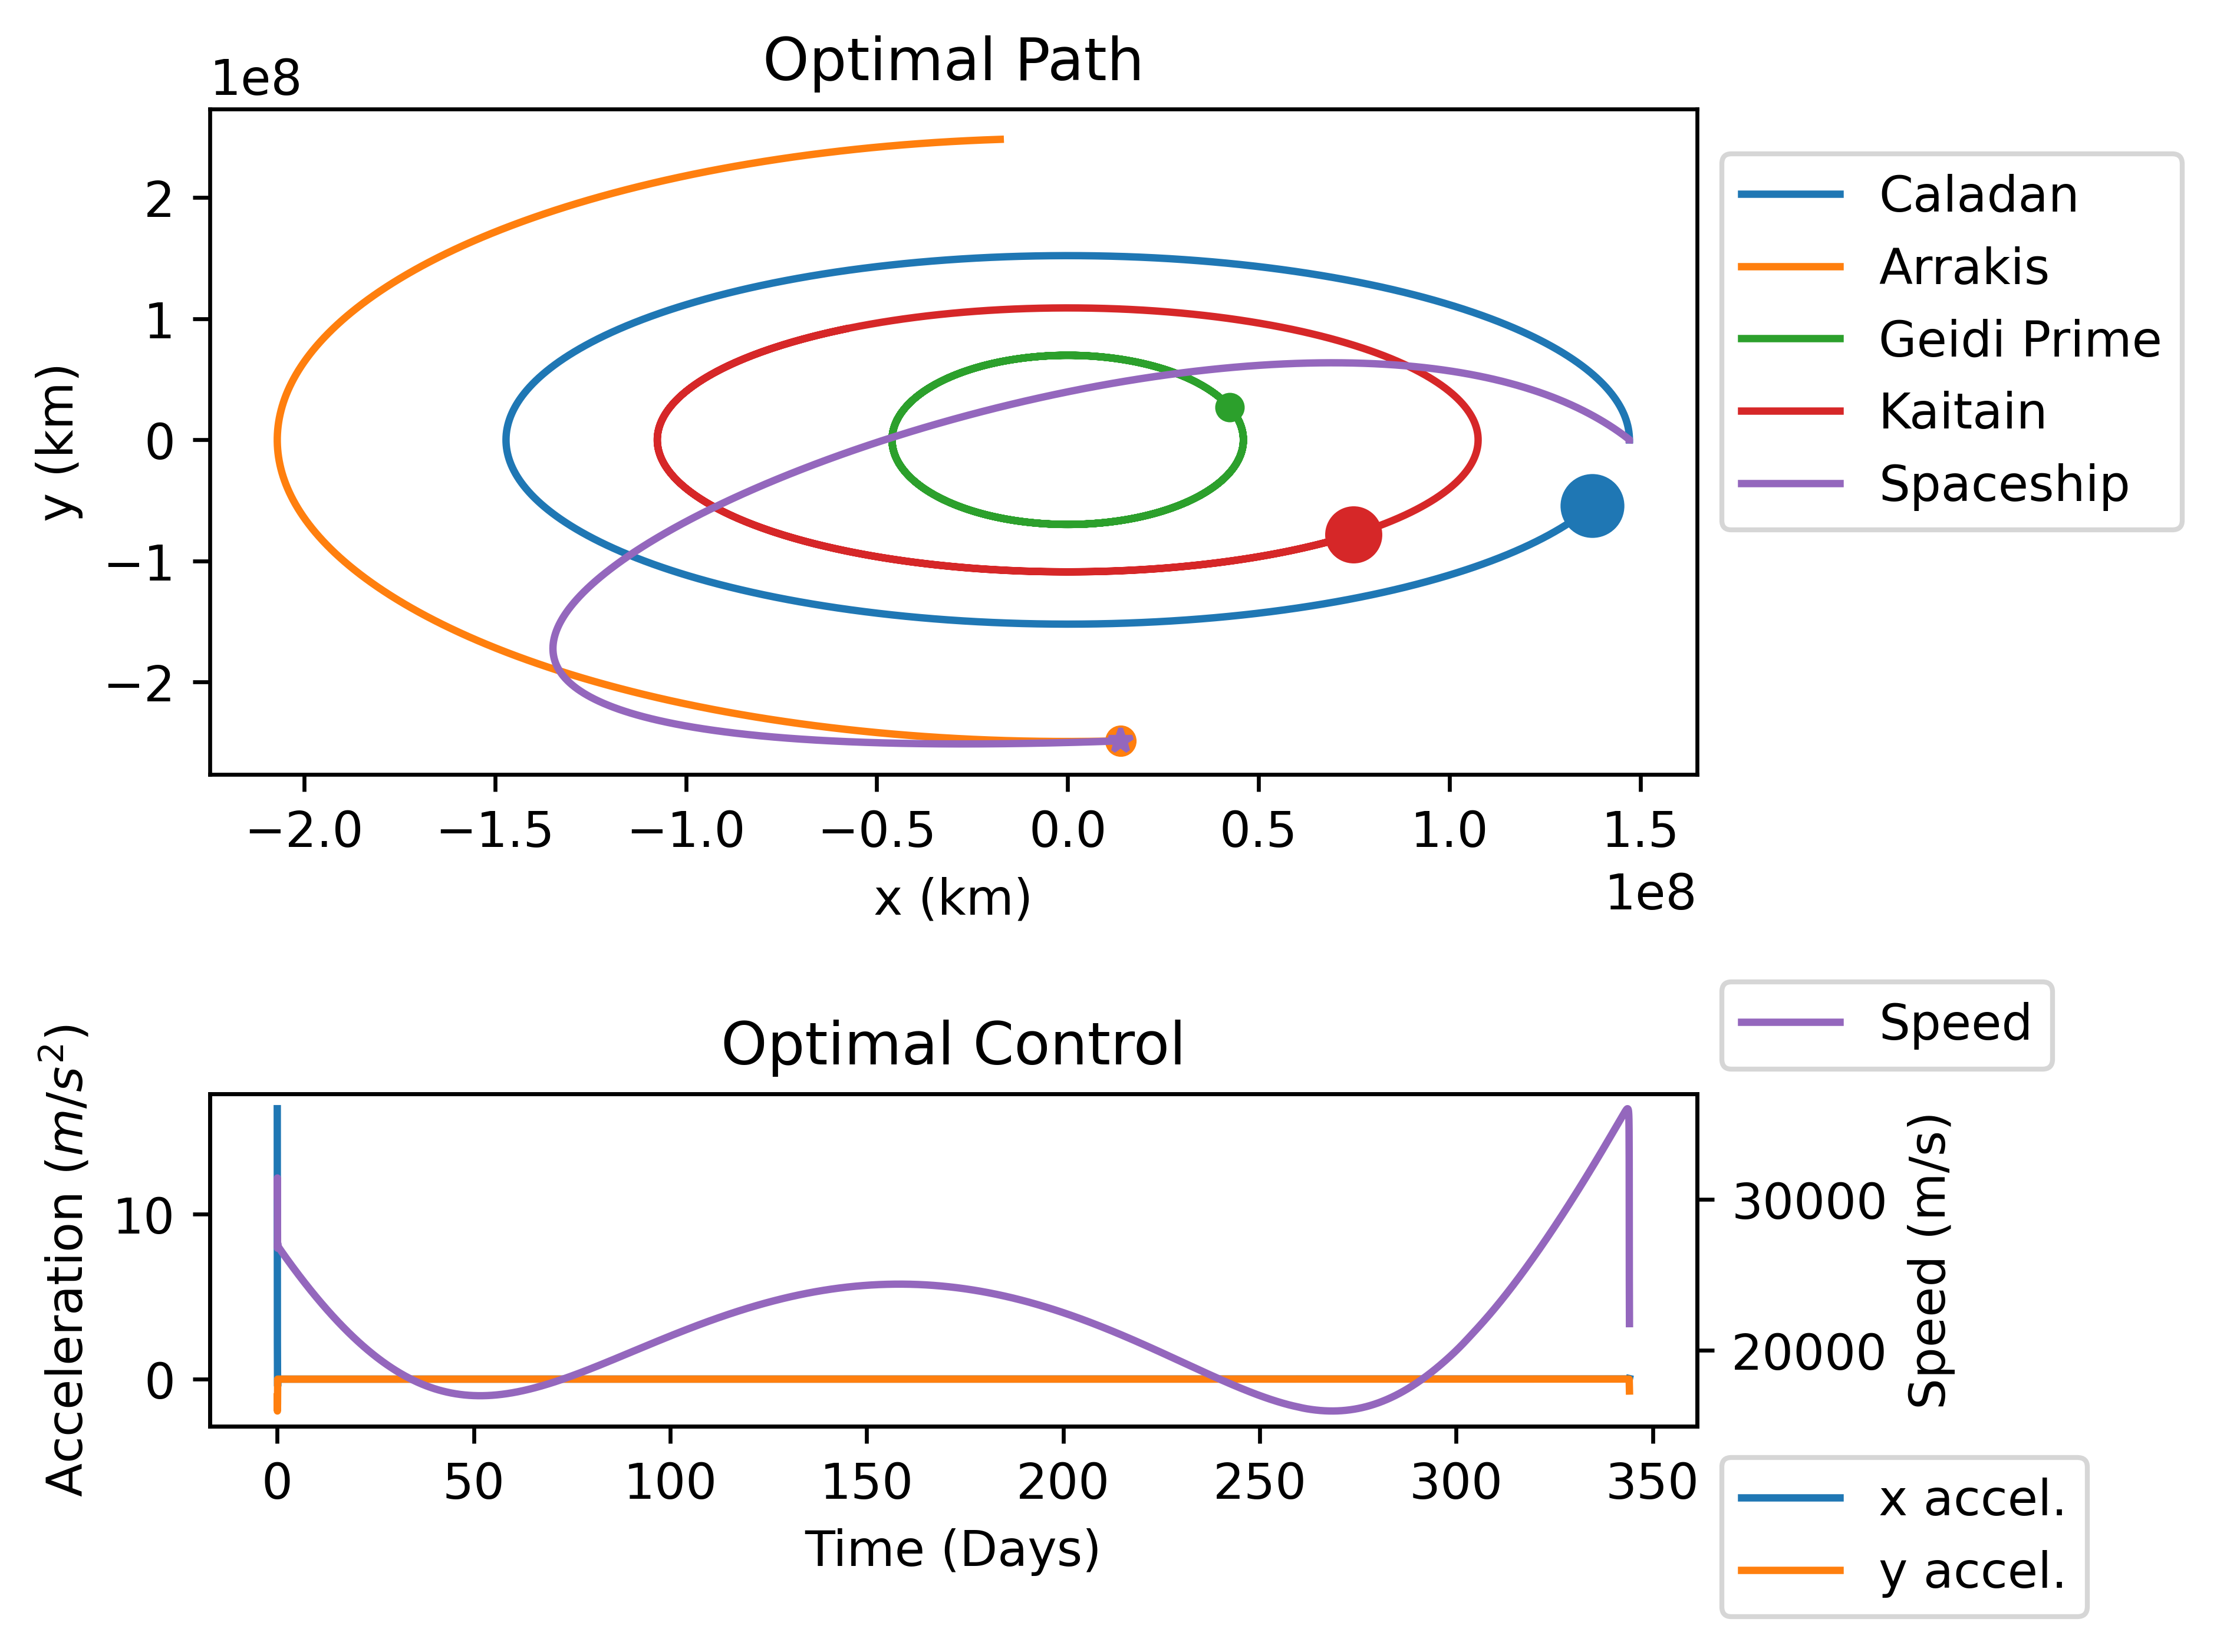
\includegraphics[width=0.8\textwidth]{f5.png}\hfill
    \caption{Going from Caladan to Arrakis with $t_f$ guess as $365$ days. The optimal $t_f$ was $344$ days.}
    \label{fig:free_time_no_sun}
\end{figure}

\subsection{Free Starting Time}

\subsection{Problems Encountered}

We needed to add the sun, but the problem became unstable due the massive size of the sun (See Figure \ref{fig:fixed_time_sun_bad}). One suggestion we had was to work in logspace and we also changed how 
we were computing the norm in the denominator. We were using a simple function that was computing the norm from the formula, but instead we started using \lstinline{scipy.linalg.norm}. These two changes 
solved the instability problem. This difference can be seen in Figure \ref{fig:fixed_time_sun_good}. One thing to notice in Figure \ref{fig:fixed_time_no_sun} and Figure \ref{fig:fixed_time_sun_good} is that the
optimal control completely changes. We believe that the control with the sun is more realistic and a control that the Guild Naviators would accept.

\begin{figure}[htp]
    \centering
    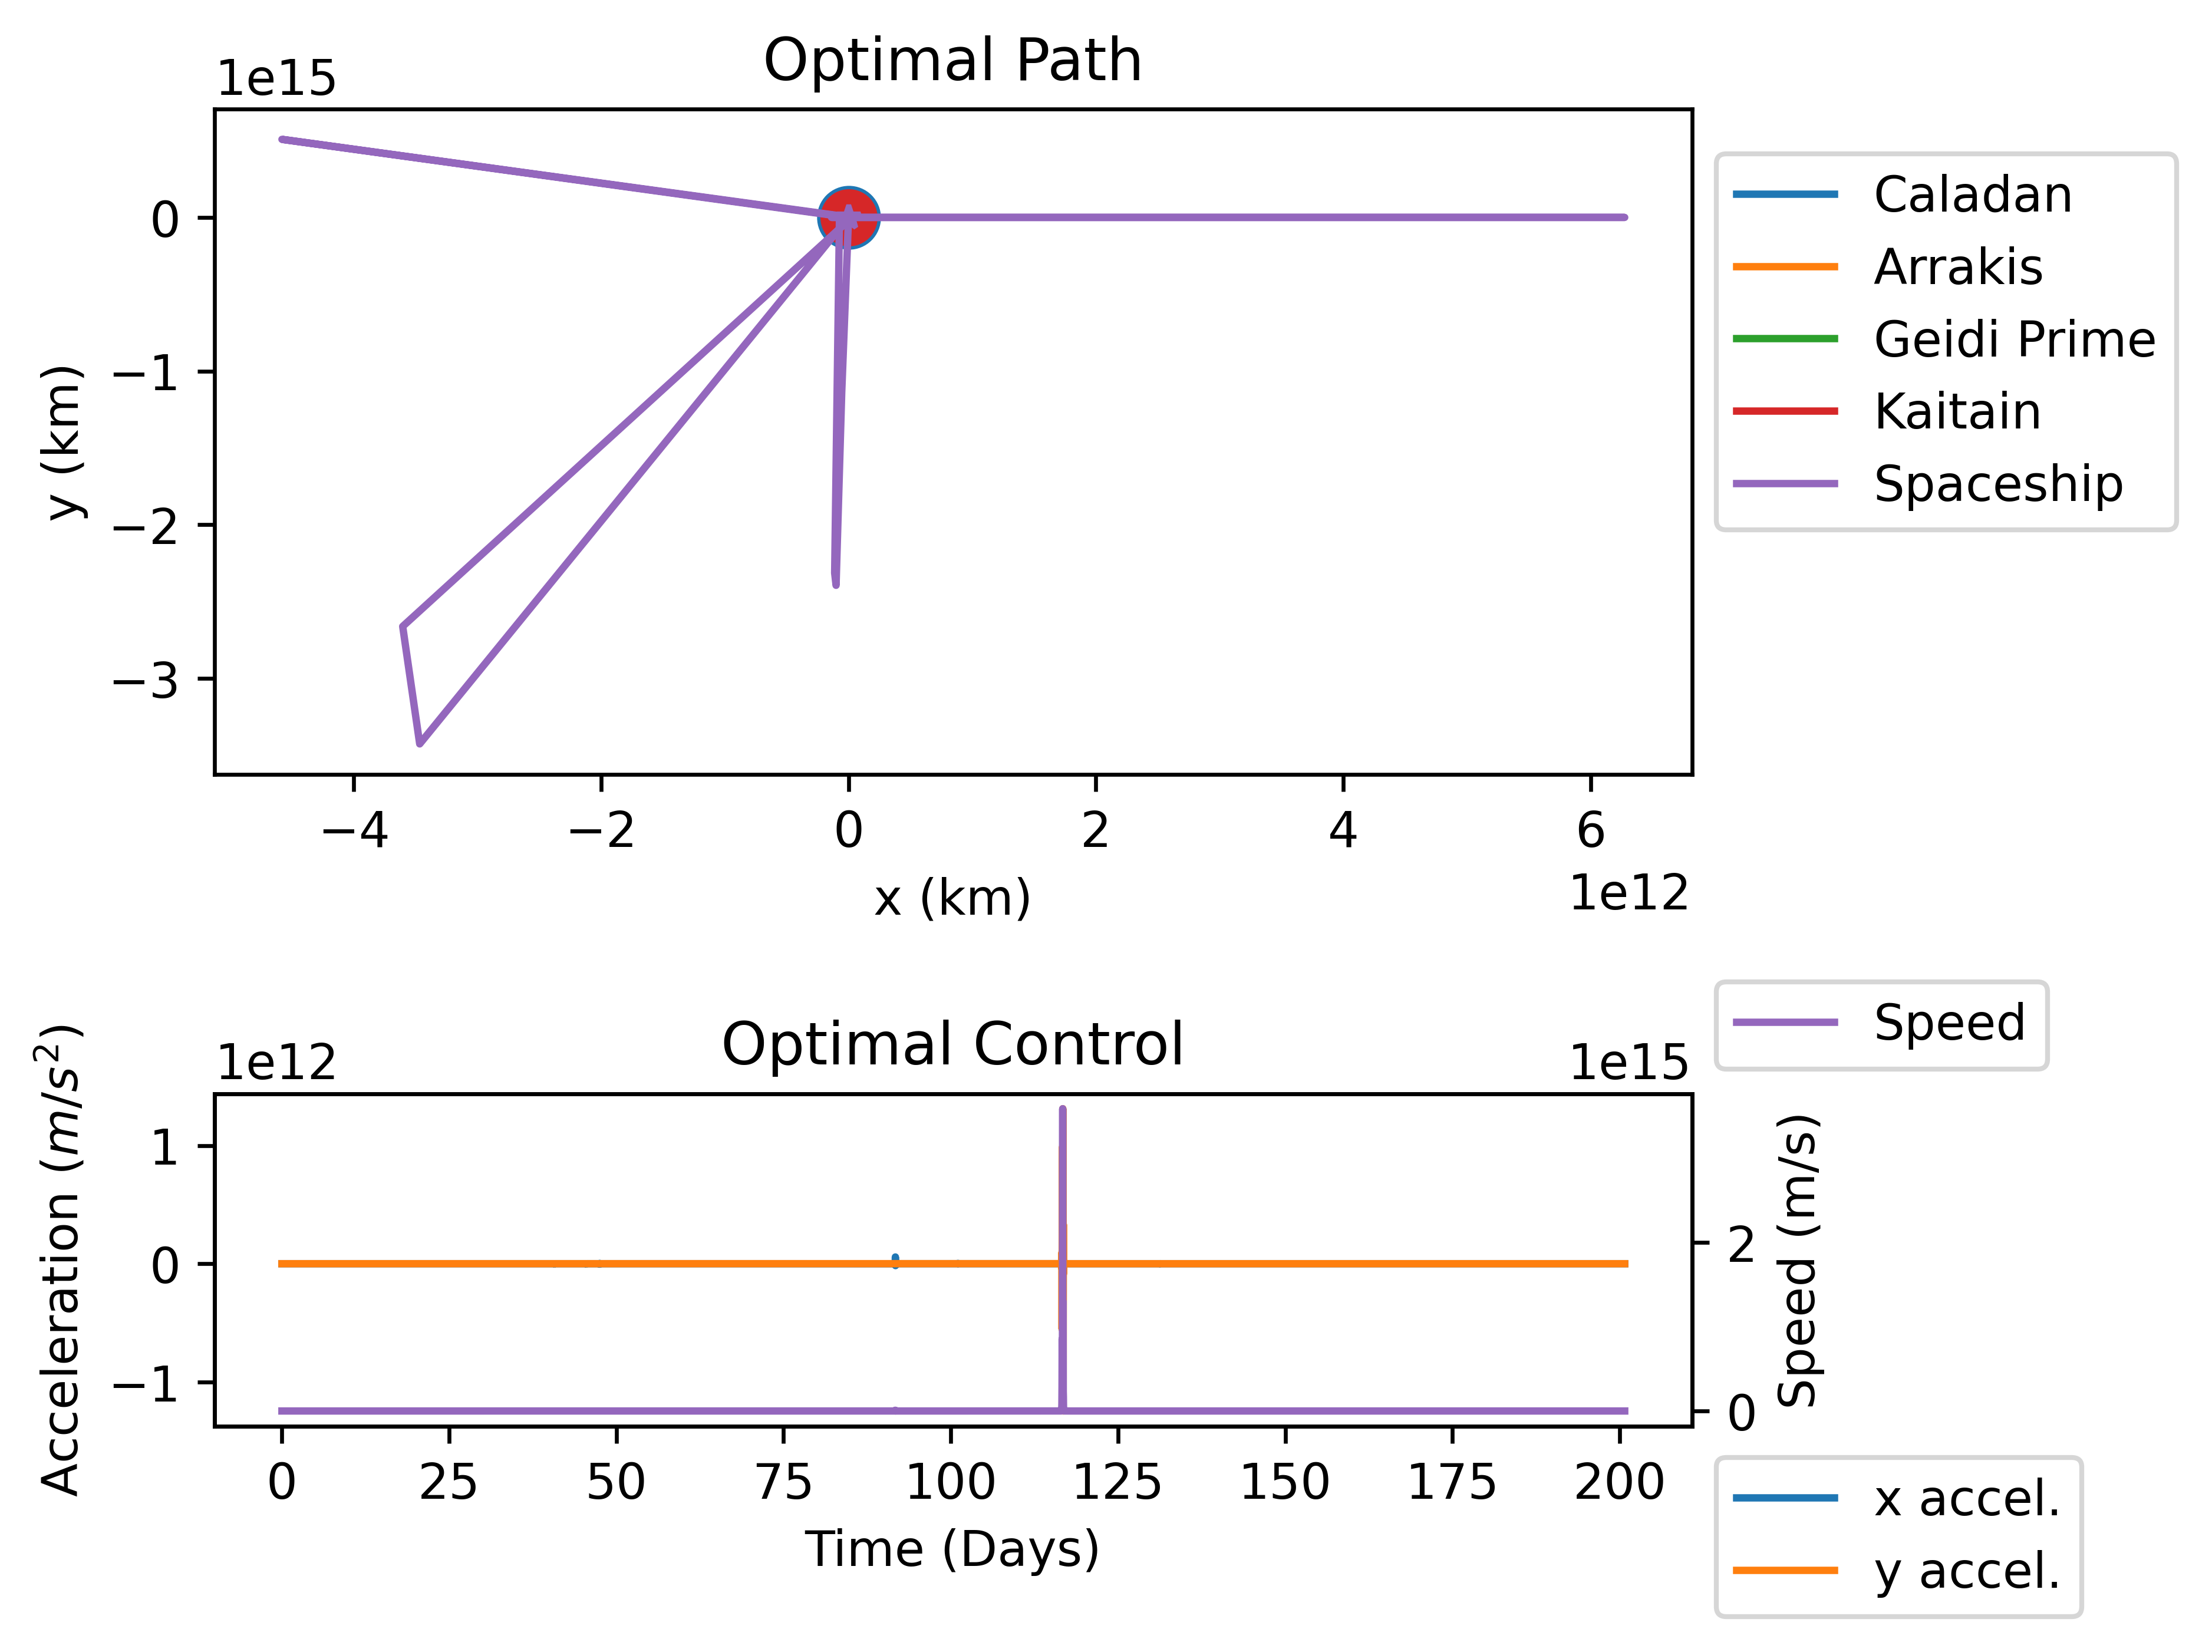
\includegraphics[width=0.8\textwidth]{instability_sun.png}\hfill
    \caption{Instability with the sun}
    \label{fig:fixed_time_sun_bad}
\end{figure}

\begin{figure}[htp]
    \centering
    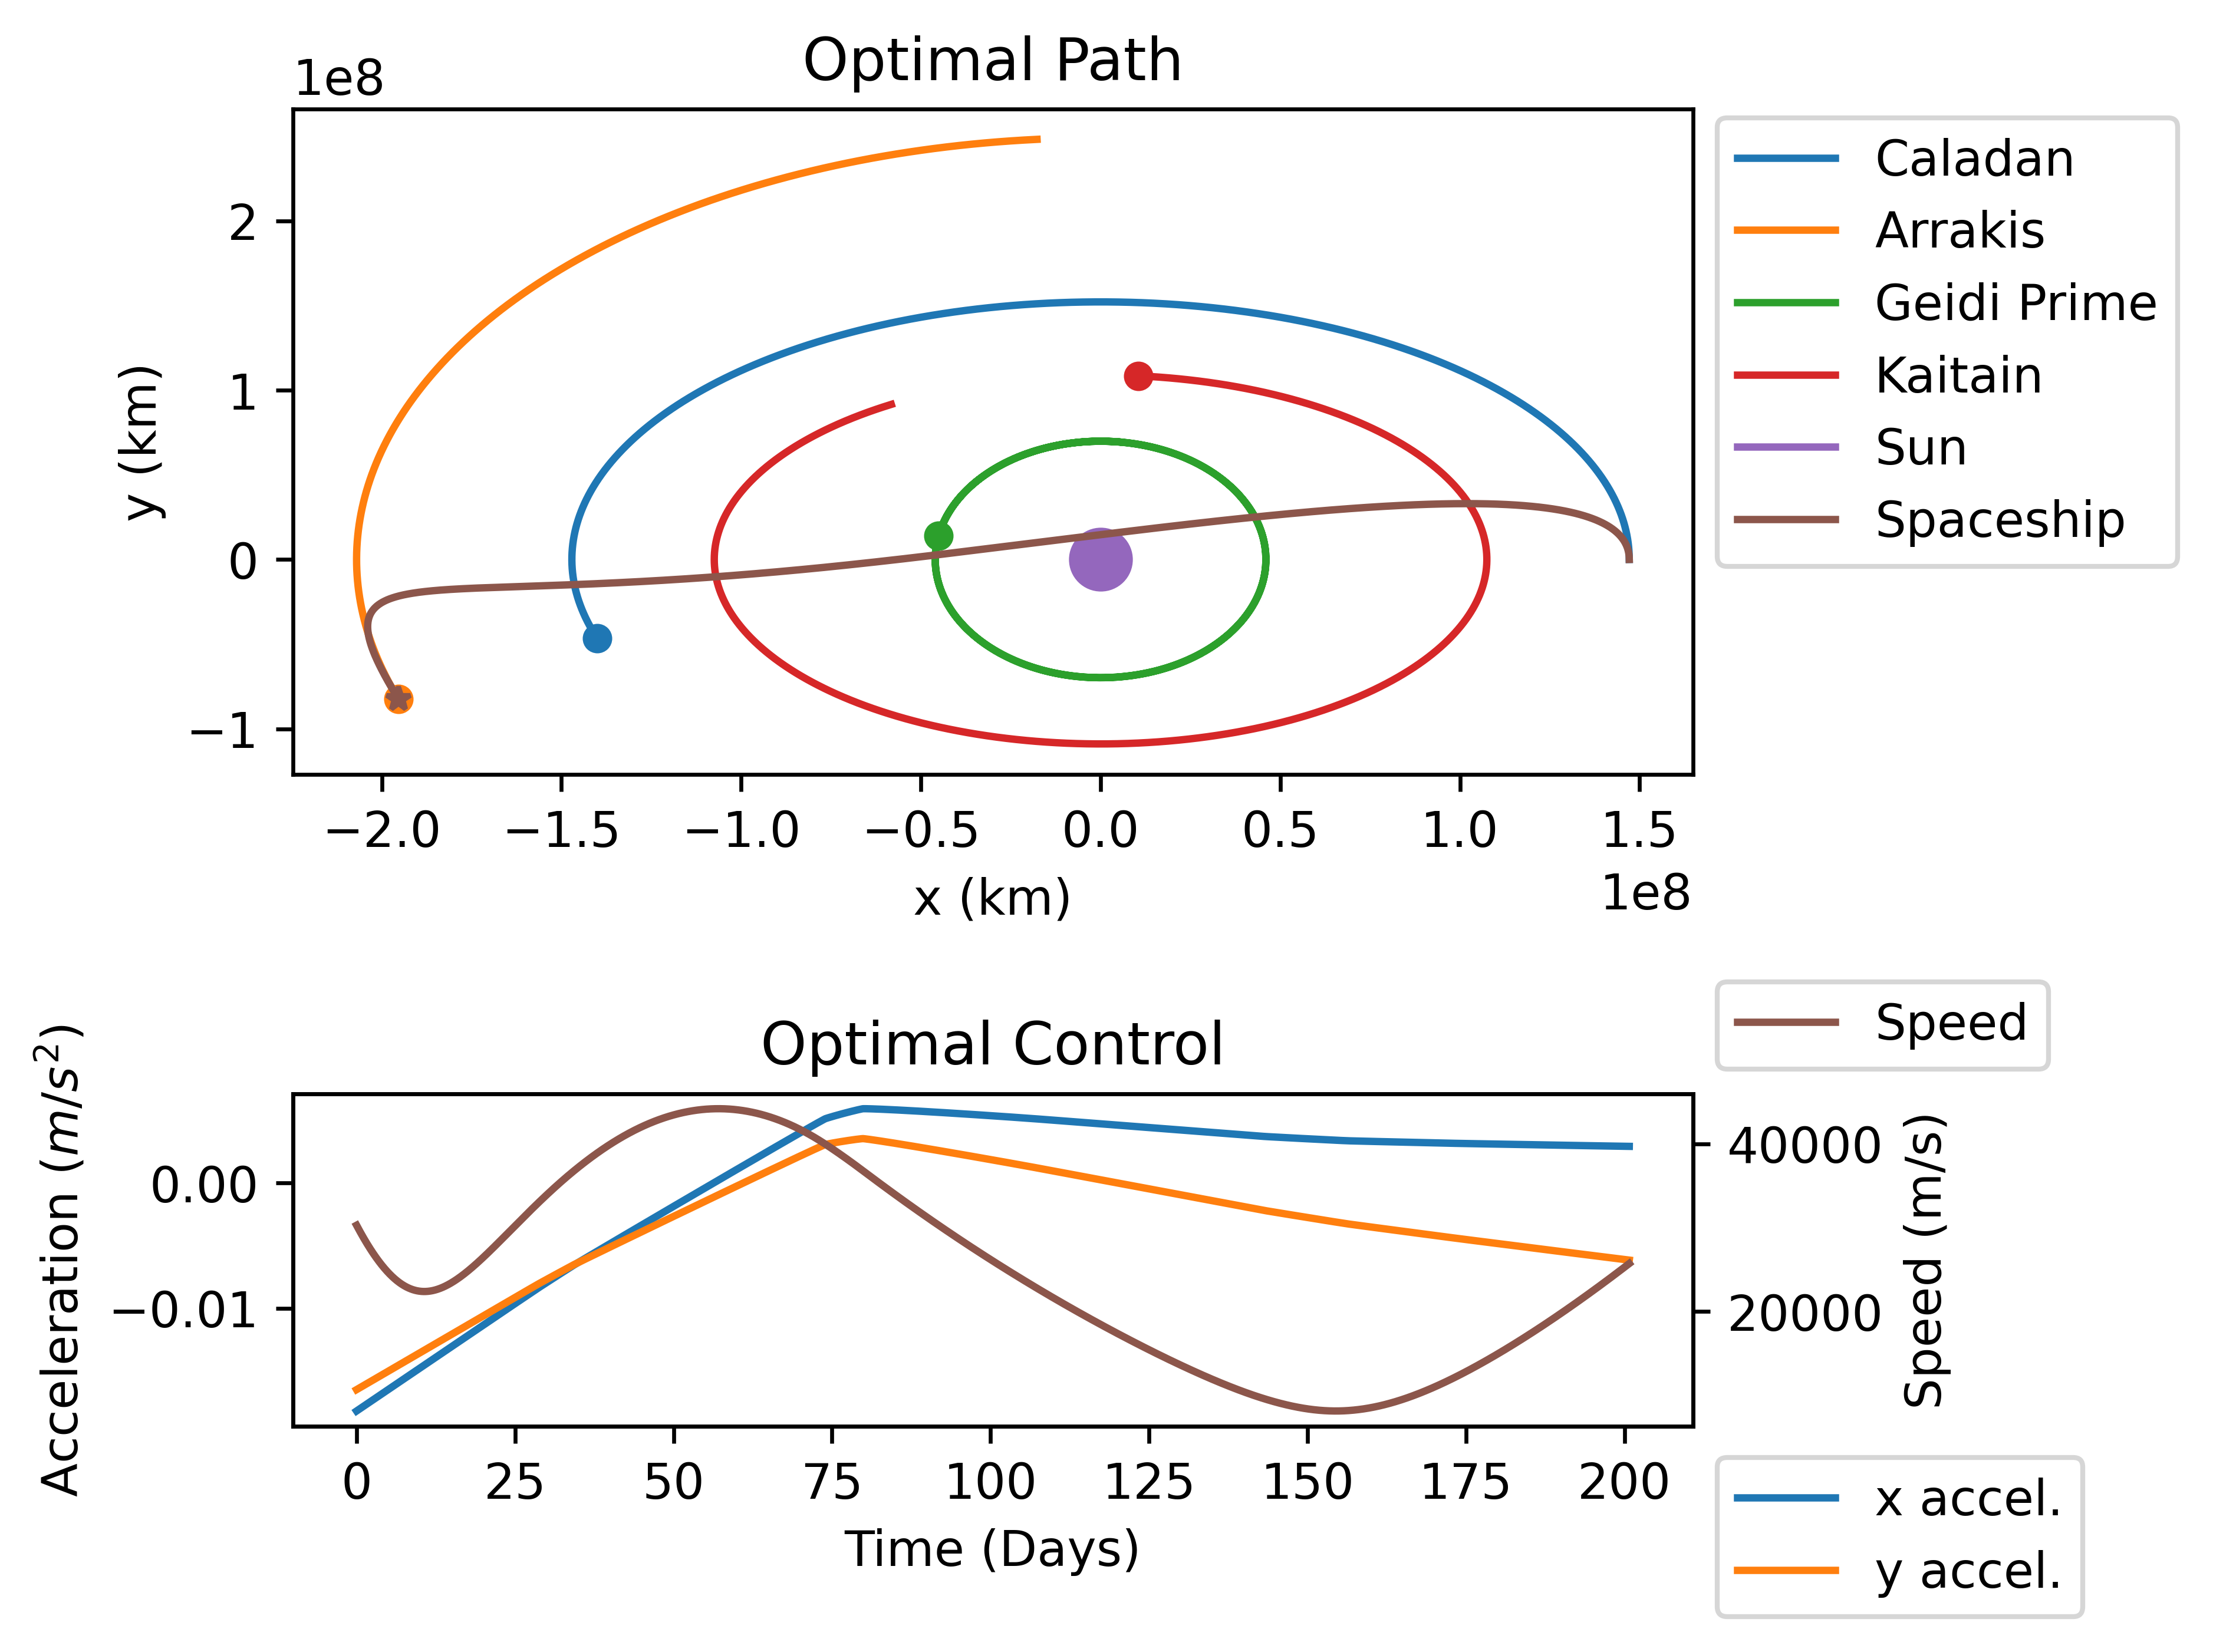
\includegraphics[width=0.8\textwidth]{f3.png}\hfill
    \caption{Stability with the sun}
    \label{fig:fixed_time_sun_good}
\end{figure}

Another problem we ran into was our units of time. Our class for planets was giving us the position of the planet in Earth years at the beginning so we thought were telling our model to get from Caladan to Arrakis in $\frac{1}{2}$ a year
by giving its final time as $\frac{1}{2}$. This was giving us an optimal control and speed that was inconceivable








%%%%%%%%%%%%%%%%%%%%%%%%%%%%%%%%%%%%%
%% Bibliography below
%%%%%%%%%%%%%%%%%%%%%%%%%%%%%%%%%%%%%
\FloatBarrier % Keep the figures from being put after the bibliography
\newpage
%% If using bibtex, leave this uncommented
%\bibliography{refs} %if using bibtex, call your bibtex file refs.bib
\bibliographystyle{alpha}

%% If not using bibtex, comment out the previous two lines and uncomment those below
\begin{thebibliography}{99}
\bibitem{Newton} William M., Samuel L., Jeff S. University Physics Volume 1. 2021 OpenStax. https://openstax.org/details/books/university-physics-volume-1 

\end{thebibliography}

\end{document}